\quad Križanjem nastaju djeca koja sadrže gene oba roditelja, ali konstantnim korištenjem istog genetskog materijala možemo postići samo određene rezultate. Mutacija nam stoji na raspolaganju kao operacija koja uvodi nove gene u populaciju. Novi geni mogu ili pospješiti ili pogoršati rezultate populacije. Ako se novi geni uvode u odgovarajućoj količini konačni učinak je pozitivan; u suprotnom je destruktivan. Promjene u bazi gena nas mogu izbaciti iz neoptimalnih rješenja u kojima bi inače ostali. Mutacija je jako korisna i važna operacija u genetskim algoritmima, ali ona je još značajnija u CGP-u gdje se koristi kao primarna genetska operacija s obzirom na nepouzdane rezultate križanja. U ovom poglavlju opisujemo mutaciju u CGP-u, utjecaj operacije na funkcioniranje mreže i načine implementacije.
\par 
Mutacija u CGP-u podrazumijeva odabir nasumičnih gena u mreži te njihovu izmjenu u neku drugu valjanu vrijednost. S obzirom na to da su geni samo adrese funkcija ili parametara možemo ih izmijeniti u drugu valjanu adresu. Kako bi adresa bila valjana mora poštivati pravila koja smo definirali u poglavlju 4: funkcijski geni smiju poprimiti samo vrijednosti adresa navedenih u tablici funkcija, geni veza ne smiju poprimiti vrijednost adresa čvorova iz stupca u kojem se nalaze ili iz stupaca desno od njih, izlazni geni mogu poprimiti adresu bilo kojeg čvora ili ulaza. Postupak je donekle sličan inicijalizaciji programa, ali na razini zasebnih gena.
\par 
Izmjena jednog ili nekoliko gena u mreži može imati puno veći utjecaj nego što bi se očekivalo u običnom genetskom programiranju. Pošto imamo kodirajuće i nekodirajuće gene moramo razmatrati utjecaj mutacije na obje vrste.
\par 
 Kod mutacije kodirajućeg gena, posebice kodirajućeg gena veze ili izlaznog gena, može doći do velike promjene fenotipa. Geni koji su prije bili nekodirajući mogu postati kodirajući, a kodirajući geni  mogu postati nekodirajući kroz samo malu promjenu toka podataka od ulaza do izlaza u mrežu. Na slikama 7.1 i 7.2 možemo vidjeti primjer promjene fenotipa uz prikaz logičkih sklopova kao načina bolje vizualizacije promjene. Pune linije predstavljaju kodirajuće gene, a isprekidane linije predstavljaju nekodirajuće gene. 
 
  \begin{figure}[h]
 	\centering
 	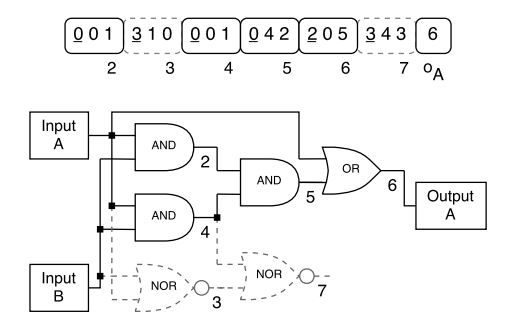
\includegraphics[width=0.5\linewidth]{pre_mutation}
 	\caption{Logički sklop prije mutacije izlaznog gena \cite{CGPbook}}
 \end{figure} 
 \begin{figure}[h]
	\centering
	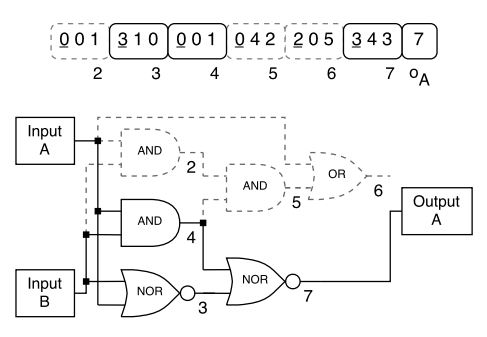
\includegraphics[width=0.5\linewidth]{post_mutation}
	\caption{Logički sklop nakon mutacije izlaznog gena iz 6 u 7 \cite{CGPbook}}
\end{figure}
\par
Mutacija nekodirajućeg gena na prvu ne pokazuje rezultate, ali je iznimno bitna. Pokazali smo kako izmjena gena fenotipa može bitno utjecati na sastav fenotipa tako da nekodirajući geni postanu kodirajući. Prema tome, svaki nekodirajući gen ima šansu postati kodirajući i sve izmjene nad njim mogu postati korisne ili štetne za rad programa. Iako nam učinak izmjene nije poznat u trenutku uspoređivanja, ovo je jedan od razloga zbog kojih u elitizmu i selekciji odabiremo djecu, a ne roditelje, ako se ispostavi da imaju jednaku dobrotu \cite{CGPbook}\cite{CGPpresentation}. 
\par
Jedan od oblika implementacije mutacije programa izmjena je nasumičnih gena dok se ne izmijeni određen postotak genotipa \cite{CGPbook}. Postotak određuje osoba koja radi implementaciju. Prilikom određivanja postotka važno je imati na umu da prevelika mutacija dovodi do destruktivnih posljedica za populaciju programa. 
\par
"Single mutation" naziv je za implementaciju mutacije gdje se izmjena gena provodi dok se ne izmjeni kodirajući gen \cite{CGPpresentation}. Ova implementacija cilja na promjenu fenotipa i ne postoji ograničenje na broj izmjena koje će se izvesti do ispunjenja uvjeta. 